% % % % % % % % % % % % % % % % % % % % % % % % % % % % % % % % % % % % % % % % 
\section{The Patmos Compiler}
\label{sec:the_patmos_compiler}

The principal components of the tool chain currently are:
(1) the C frontend \texttt{Clang},\footnote{\url{http://clang.llvm.org/}} (2)
the LLVM optimisers, (3) an LLVM-based code generator and LLVM-based utilities
for the Patmos processor, (4) the \texttt{gold} linker of the binutils project,%
\footnote{\url{http://sourceware.org/binutils/}} (5) the \texttt{newlib} C
library,\footnote{\url{http://sourceware.org/newlib/}} and (6) the compiler
support library \texttt{compiler-rt}.%
\footnote{\url{http://compiler-rt.llvm.org/}}

\subsection{Tool Chain Overview}
\label{sec:toolchain_overview}

Figure~\ref{fig:framework} depicts a typical compilation flow of the Patmos
tool chain. First, the C source code of a user-supplied application is
translated to LLVM bitcode using the \texttt{clang} frontend. Next, the
generated bitcode files are linked with the system libraries (e.g., the 
\texttt{newlib} C library) using the LLVM tool \texttt{llvm-ld}. This results in
one combined bitcode file, which contains all user- and system code of the
application. The \emph{linked} application can then be optimised using the
high-level optimisations of LLVM, which are readily available through
\texttt{llvm-ld}. In the following step the linked and optimised bitcode is
translated to machine code using the Patmos code generator and the LLVM tool
\texttt{llc}. This results in a relocatable ELF binary, which already contains
the entire machine code of the application and thus is, in principle, ready to
be executed. The final step of the tool chain performs the final code and data
layout of the application using the \texttt{gold} linker and an optional,
user-supplied linker script. Note that no new code is added at this step since
all libraries were already linked at the bitcode-level beforehand. This
compilation flow was specifically designed to facilitate the development of
future WCET-driven compilation techniques within the T-CREST project. Since all
the application code is linked into a single bitcode file, the LLVM optimisers
and the Patmos code generator have a complete view of all the application code
needed to optimise the WCET.

\begin{figure}[t]
  \centering
  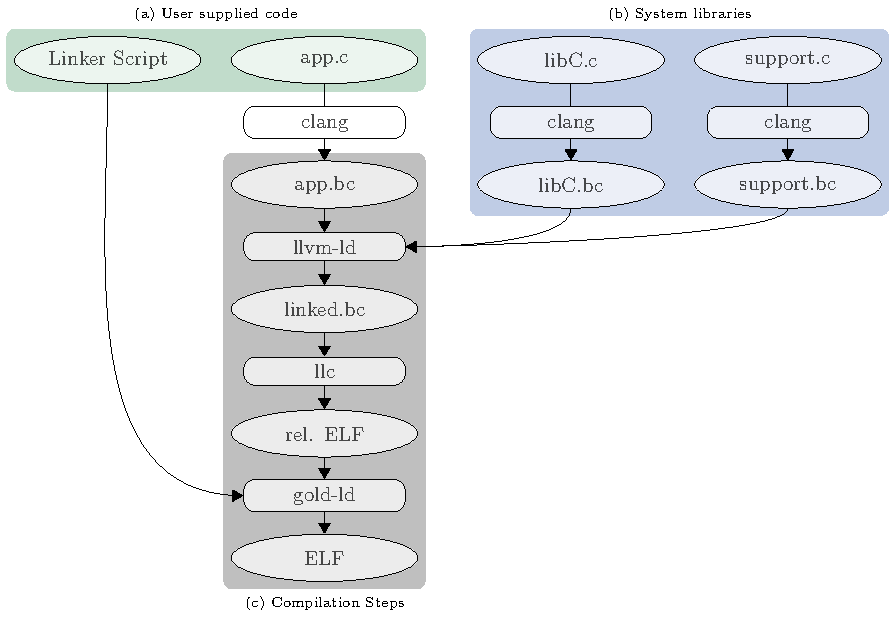
\includegraphics{fig/framework}

  \caption{Compilation flow of the Patmos tool chain.}
  \label{fig:framework}
\end{figure}

The following section describes each of these components in more detail.

% ------------------------------------------------------------------------------
\subsection{Principal Components}

% TODO:
%   clang, llvm-ld, llc, gold, newlib, compiler-rt
%   mention LLVM generated assembler and disassembler
%   simulator?

\begin{description}
\item[clang] \hfill\\
  \texttt{clang} is the C frontend that translates source code files written in C
  to the LLVM intermediate representation (aka \emph{bitcode}). The bitcode
  is the representation the LLVM analyses and optimisations work upon.
  \texttt{clang} also acts as a driver that invokes the tools involved with the
  options specific for targeting Patmos.

  \begin{tabular}{ll}
  Input:  & \texttt{.c} source code file \\
  Output: & \texttt{.bc} bitcode object file
  \end{tabular}

\item[llvm-ld] \hfill\\
  \texttt{llvm-ld} links bitcode files and static libraries of bitcode files
  together into a bitcode file containing the bitcode from the input files
  and the required symbol definitions from the libraries.

  \begin{tabular}{ll}
  Input:  & \texttt{.bc} bitcode object files [, \texttt{lib*.a} bitcode
            libraries ]\\
  Output: & \texttt{.bc} linked bitcode object file
  \end{tabular}

\item[llc] \hfill\\
  \texttt{llc} constitutes the backend translating a bitcode file into either
  assembly or binary machine code for the Patmos ISA.
  The binary output format is relocatable ELF.

  \begin{tabular}{ll}
  Input:  & \texttt{.bc} bitcode object file \\
  Output: & \texttt{.s} Patmos assembly \\
          & or \texttt{.o} Patmos relocatable ELF
  \end{tabular}

\item[gold] \hfill\\
  \texttt{gold} is an ELF linker.
  In our tool chain it is adopted to perform relocations.

  \begin{tabular}{ll}
  Input:  & \texttt{.o} Patmos relocatable ELF \\
  Output: & \texttt{.o} Patmos final ELF
  \end{tabular}

\item[C Library] \hfill\\
  We adopted \texttt{newlib}, a
  standard ANSI C library following the C90 and C99 
  standards~\cite{ISO:9899:1990,ISO:9899:1999}, for Patmos. In the Patmos 
  compilation flow the entire \texttt{newlib} C library is translated to LLVM 
  bitcode and linked as such with the application program \emph{before} code 
  generation. This is an important precondition for WCET-driven compilation as 
  envisioned in the T-CREST project, as it provides the compiler with a complete 
  view of \emph{all} code belonging to an application.

\item[Support Library] \hfill\\
  The LLVM compiler requires a support library, which provides for instance 
  emulation functions for floating-point operations. LLVM's 
  \texttt{compiler-rt} support
  library has been adopted for Patmos and is, similar to the C library, compiled 
  to LLVM bitcode and linked with the application program if needed.
\end{description}

